\documentclass[tikz]{standalone}
\usepackage{pgfplots}
\pgfplotsset{compat=1.15}
\usepackage{mathrsfs}
\usetikzlibrary{arrows,calc}
\usepackage{tkz-euclide}

\pagestyle{empty}

\definecolor{AngleClr}{rgb}{0,0.39215686274509803,0}
\definecolor{ShapeClr}{rgb}{0.6,0.2,0}

\begin{document}

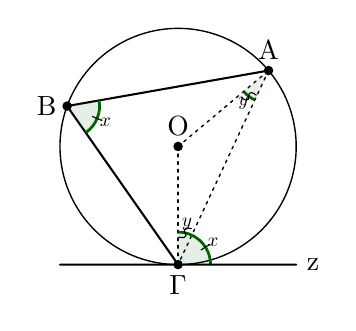
\begin{tikzpicture}[scale=.75]
\tkzSetUpLine[line width=1pt,color=black]
\tkzSetUpPoint[fill=black]

\tkzDefPoints{0/0/O,2/0/X}

\tkzDefPoint(-90:2){C}
\tkzDefPoint(40:2){A}
\tkzDefPoint(160:2){B}

\tkzDrawSegments[line width=0.75pt,color=black](A,B C,B)
\tkzDrawSegments[line width=0.5pt,color=black,dashed,dash pattern=on 1pt off 1.75pt](O,C A,C O,A)

\tkzDrawCircle[color=black,line width=0.5pt](O,X)

\tkzDefLine[tangent at=C](O)
\tkzGetPoint{h}

\tkzFillAngles[fill=AngleClr,size=.55,fill opacity=0.1](C,B,A h,C,A)
\tkzMarkAngles[mark=|,mksize=2,line width=1pt,size=.55,color=AngleClr](C,B,A h,C,A)
\tkzLabelAngle[scale=0.7](C,B,A){$x$}
\tkzLabelAngle[scale=0.7](h,C,A){$x$}

\tkzFillAngles[fill=AngleClr,size=.55,fill opacity=0.1](O,A,C A,C,O)
\tkzMarkAngles[mark=s,mksize=2,line width=1pt,size=.55,color=AngleClr](O,A,C A,C,O)
\tkzLabelAngle[scale=0.7](O,A,C){$y$}
\tkzLabelAngle[scale=0.7](A,C,O){$y$}


\tkzDrawSegments[line width=0.75pt,color=black,add=2 and 1](C,h)
\tkzDrawPoints[size=3](A,B,C,O)
\tkzLabelPoint[above](A){$\rm A$}
\tkzLabelPoint[left](B){$\rm B$}
\tkzLabelPoint[below](C){$\rm \Gamma$}
\tkzLabelPoint[above](O){$\rm O$}
\tkzLabelPoint[right=0.75cm](h){$\rm z$}


\end{tikzpicture}

\end{document}
